\documentclass[border=5pt,convert={outfile=../_static/\jobname.svg}]{standalone}

\usepackage[T1]{fontenc}
\usepackage[default]{raleway}

\usepackage{tikz}
    \usetikzlibrary{%
        arrows,
        decorations.pathreplacing,
        positioning,
        shapes,
        shapes.geometric}

\tikzstyle{every picture} += [remember picture]

\tikzset{%
    column/.pic={code{%
    \draw[line width=1pt]
        (0, 0) -- ++(0, 4cm) -- ++(-2cm, 0) -- ++(0, -4cm);
    \foreach \val in {0, ..., #1}{%
        \draw[rotate=90] ([xshift=-\val*10pt] 4cm, 2cm) -- ++(0, -2cm);
    };
    \node at (-1, 0.75) {$\vdots$};
    }}
}

\begin{document}

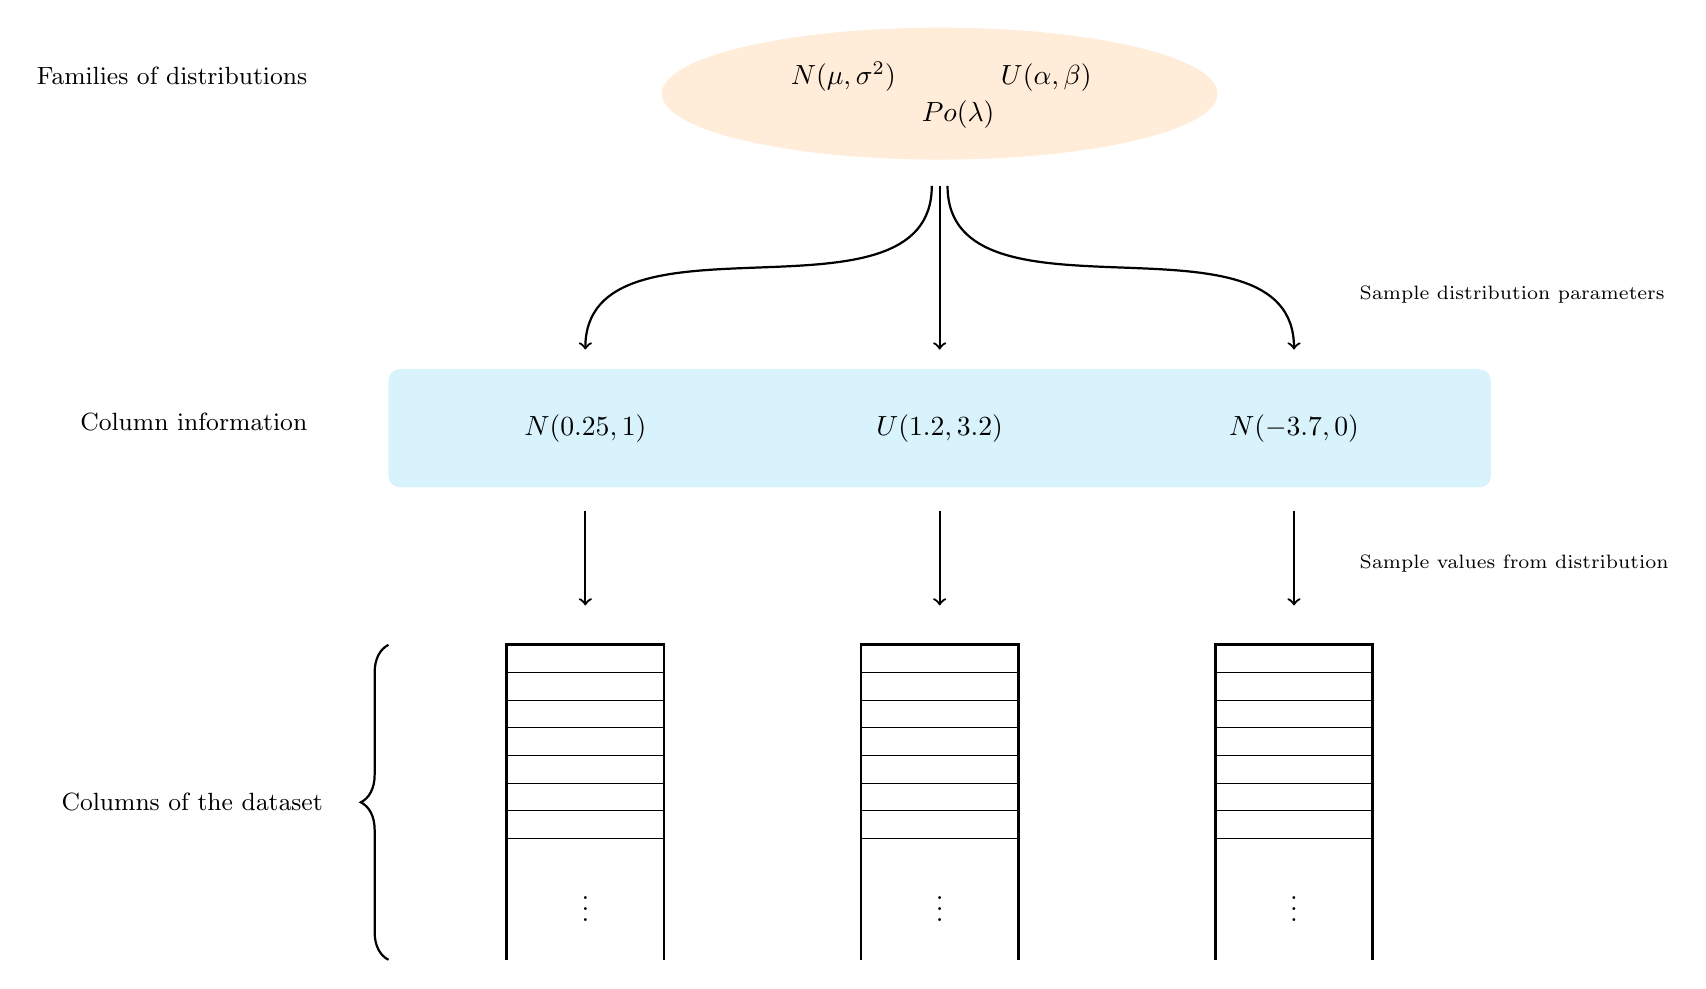
\begin{tikzpicture}

    \path (-3.5, -10) pic {column=7}
          (1, -10) pic {column=7}
          (5.5, -10) pic {column=7};

    \node[ellipse, fill=orange!15] (dists) at (0, 1) {%
        \begin{tabular}{c}
            \tikz[baseline, inner sep=0] \node[anchor=base] (normal) {$N(\mu,
            \sigma^2)$}; \quad \quad \tikz[baseline, inner sep=0]
            \node[anchor=base] (uniform) {$U(\alpha, \beta)$}; \\
            {} \quad $Po(\lambda)$
        \end{tabular}
    } node[yshift=35pt, left=225pt] {\small Families of distributions};

    \fill[cyan!15, rounded corners] node[yshift=-90pt, left=225pt]
        {\color{black} \small Column information} (-7, -4) rectangle
        (7, -2.5);
    
    \node (norm1) at (-4.5, -3.25) {$N(0.25, 1)$};
    \node (norm2) at (4.5, -3.25) {$N(-3.7, 0)$};
    \node (uniform1) at (0, -3.25) {$U(1.2, 3.2)$};

    \draw[->, thick] ([xshift=-0.1cm] normal.south) to [out=270, in=90]
        ([yshift=1cm] norm1);
    \draw[->, thick] ([yshift=-0.75cm] norm1.south) -- (-4.5, -5.5);

    \draw[->, thick] ([xshift=0.1cm] normal.south) to [out=270, in=90]
        ([yshift=1cm] norm2) node[right=20pt, yshift=20pt] {%
        \scriptsize Sample distribution parameters
    };
    \draw[->, thick] ([yshift=-0.75cm] norm2.south) -- (4.5, -5.5)
        node[right=20pt, yshift=15pt] {%
        \scriptsize Sample values from distribution
    };
    \draw[->, thick] (uniform) to [out=270, in=90] ([yshift=1cm] uniform1);
    \draw[->, thick] ([yshift=-0.75cm] uniform1.south) -- (0, -5.5);

    \draw[decorate, decoration={brace, amplitude=10pt}, thick] (-7, -10) -- (-7, -6)
    node[midway, left=20pt] {\small Columns of the dataset};

\end{tikzpicture}

\end{document}
